

\section{OpticalElement: \textquotedbl{}MICADO\_SCAO\textquotedbl{}%
  \label{opticalelement-micado-scao}%
}

\textbf{Element}: instrument

\textbf{Alias}: INST

\textbf{Description}: MICADO SCAO mode effects


\subsection{Global properties%
  \label{global-properties}%
}

\begin{quote}
\begin{alltt}
\begin{lstlisting}[frame=single]
         psf : \{'strehl': 0.8, 'wavelength': 'Ks'\}
element_name : MICADO_SCAO
\end{lstlisting}
\end{alltt}
\end{quote}


\subsection{Effects%
  \label{effects}%
}

Summary of Effects included in this optical element:

\setlength{\DUtablewidth}{\linewidth}
\begin{longtable*}[c]{|p{0.145\DUtablewidth}|p{0.261\DUtablewidth}|p{0.214\DUtablewidth}|p{0.110\DUtablewidth}|p{0.179\DUtablewidth}|}
\hline
\textbf{%
element
} & \textbf{%
name
} & \textbf{%
class
} & \textbf{%
included
} & \textbf{%
z\_orders
} \\
\hline
\endfirsthead
\hline
\textbf{%
element
} & \textbf{%
name
} & \textbf{%
class
} & \textbf{%
included
} & \textbf{%
z\_orders
} \\
\hline
\endhead
\multicolumn{5}{c}{\hfill ... continued on next page} \\
\endfoot
\endlastfoot

MICADO\_SCAO
 & 
scao\_relay\_optics\_ter
 & 
TERCurve
 & 
True
 & 
{[}10, 110, 510{]}
 \\
\hline

MICADO\_SCAO
 & 
scao\_const\_psf
 & 
AnisocadoConstPSF
 & 
True
 & 
{[}42, 652{]}
 \\
\hline
\end{longtable*}
\label{tbl-micado-scao}


\subsubsection{TERCurve: \textquotedbl{}scao\_relay\_optics\_ter\textquotedbl{}%
  \label{tercurve-scao-relay-optics-ter}%
}

\textbf{Included by default}: \texttt{True}

\textbf{File Description}: Combined TER curve for stand-alone relay optics module

\textbf{Class Description}: Transmission, Emissivity, Reflection Curve

\textbf{Changes}:

\begin{itemize}
\item \end{itemize}


\paragraph{Data%
  \label{data}%
}

\begin{figure}[H]
\noindent\makebox[\linewidth][c]{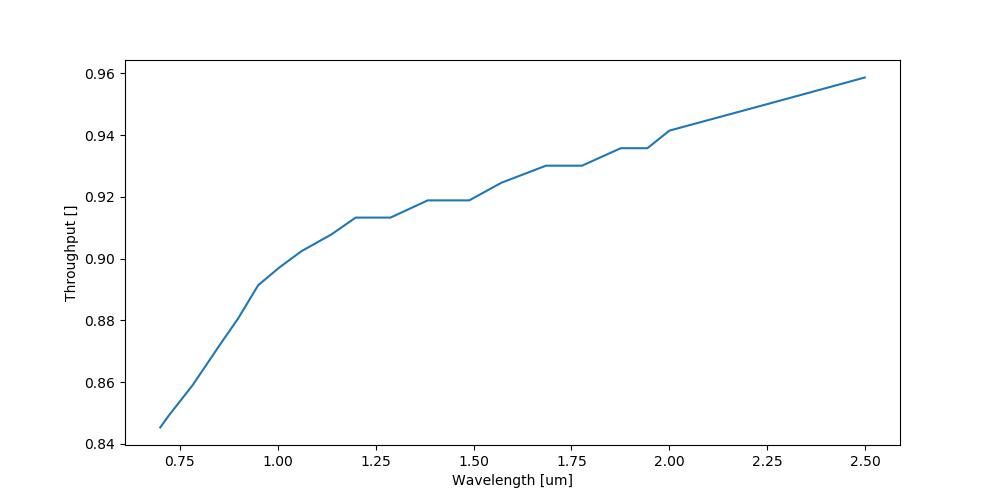
\includegraphics{scao_relay_optics_ter.png}}\phantomsection\label{fig-scao-relay-optics-ter}
\end{figure}


\paragraph{Meta-data%
  \label{meta-data}%
}

\begin{quote}
\begin{alltt}
\begin{lstlisting}[frame=single]
            filename : TER_MICADO_RO.dat
                name : scao_relay_optics_ter
                 psf : \{'strehl': 0.8, 'wavelength': 'Ks'\}
        element_name : MICADO_SCAO
              author : Auto-compiled from source
              source : LIST_RO_SCAO_mirrors.dat
        date_created : 2020-08-25
       date_modified : 2020-08-25
                area : 0.22061834409834324
           area_unit : m2
     wavelength_unit : um
       emission_unit : photlam
             z_order : [10, 110, 510]
             include : True
        ignore_wings : False
            wave_min : 0.7
            wave_max : 2.5
           wave_unit : um
            wave_bin : 0.001
 report_plot_include : True
report_table_include : False
\end{lstlisting}
\end{alltt}
\end{quote}


\subsubsection{AnisocadoConstPSF: \textquotedbl{}scao\_const\_psf\textquotedbl{}%
  \label{anisocadoconstpsf-scao-const-psf}%
}

\textbf{Included by default}: \texttt{True}

\textbf{File Description}: field constant PSF as produced by stand-alone SCAO

\textbf{Class Description}: Makes a SCAO on-axis PSF with a desired Strehl ratio at a given wavelength

\textbf{Changes}:

\begin{itemize}
\item \end{itemize}


\paragraph{Data%
  \label{id1}%
}

\begin{figure}[H]
\noindent\makebox[\linewidth][c]{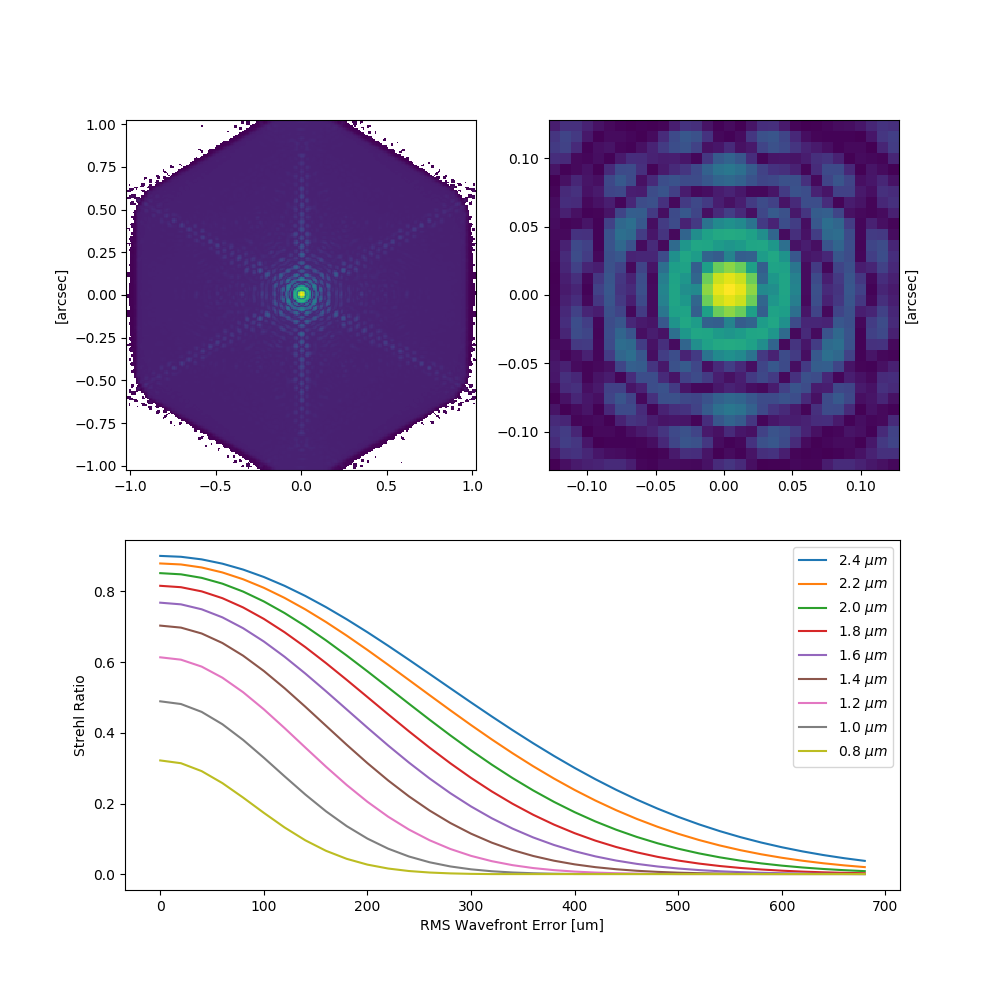
\includegraphics{scao_const_psf.png}}\phantomsection\label{fig-scao-const-psf}
\end{figure}


\paragraph{Meta-data%
  \label{id2}%
}

\begin{quote}
\begin{alltt}
\begin{lstlisting}[frame=single]
            filename : MICADO_AnisoCADO_rms_map.fits
                name : scao_const_psf
                 psf : \{'strehl': 0.8, 'wavelength': 'Ks'\}
        element_name : MICADO_SCAO
              strehl : !INST.psf.strehl
          wavelength : !INST.psf.wavelength
     psf_side_length : 256
              offset : [0, 0]
       rounded_edges : True
       convolve_mode : full
              SIMPLE : True
              BITPIX : -64
               NAXIS : 2
              NAXIS1 : 35
              NAXIS2 : 9
              EXTEND : True
              CRVAL1 : 0
              CRVAL2 : 0.8
              CRPIX1 : 1.0
              CRPIX2 : 1.0
              CDELT1 : 20
              CDELT2 : 0.2
              CUNIT1 : nm
              CUNIT2 : um
              CTYPE1 : LINEAR
              CTYPE2 : LINEAR
              LABEL1 : nmRMS
              LABEL2 : wavelength
              AUTHOR : Kieran Leschinski
            DATE_CRE : 2019-07-30
            DATE_MOD : 2019-07-30
              SOURCE : AnisoCADO
              STATUS : Strehl as a function of wavelength and wavefront error (nmRMS)
               ETYPE : SRMAP
                ECAT : -1
               EDATA : 0
             XOFFSET : 0
             YOFFSET : 0
             z_order : [42, 652]
             include : True
       flux_accuracy : 0.001
      sub_pixel_flag : False
            wave_key : WAVE0
    normalise_kernel : True
 report_plot_include : True
report_table_include : False
\end{lstlisting}
\end{alltt}
\end{quote}
